\documentclass[]{beamer}
\usepackage[utf8]{inputenc}
\usepackage{hyperref}
\usepackage{listings}
\lstset{
basicstyle=\fontsize{10}{12}\selectfont\ttfamily,
keywordstyle=\color{blue},
breaklines=true,
showtabs=false,
showstringspaces=false,
numberstyle=\tiny\color{mygray}
}
% \usepackage[french]{babel}
% \uselanguage{French}
% \languagepath{French}
\usepackage{pslatex}        % for better PDF on screen
%\usepackage{textcomp}

%\usetheme{AnnArbor}
%\usetheme{Antibes}
%\usetheme{Berkeley}
%\usetheme{Berlin}
%\usetheme{Boadilla}
\usetheme{CambridgeUS}
%\usetheme{Copenhagen}
%\usetheme{Dresden}
%\usetheme{Frankfurt}
%\usetheme{Goettingen}
%\usetheme{Hannover}
%\usetheme{JuanLesPins}
%\usetheme{Marburg}
%\usetheme{Montpellier}
%\usetheme{PaloAlto}
%\usetheme{Pittsburgh}
%\usetheme{Rochester}
%\usetheme{Singapore}
%\usetheme{Szeged}
%\usetheme{Warsaw}



% Set Color ==============================
% Custom colors tested with CambridgeUS.
% If you want a nice looking presentation,
% simply comment this section.
\usepackage{xcolor}

% http://www.computerhope.com/htmcolor.htm
\definecolor{gold}{HTML}{FDD017}
\definecolor{deep sky blue}{HTML}{3BB9FF}
\definecolor{light sky blue}{HTML}{82CAFA}
\definecolor{casesBlue}{HTML}{0072b8}

\makeatletter
\definecolor{mybackground}{HTML}{82CAFA}
\definecolor{myforeground}{HTML}{0000A0}

\setbeamercolor{normal text}{fg=black,bg=white}
\setbeamercolor{alerted text}{fg=red}
\setbeamercolor{example text}{fg=black}

\setbeamercolor{background canvas}{fg=myforeground, bg=white}
\setbeamercolor{background}{fg=myforeground, bg=mybackground}

\setbeamercolor{palette primary}{fg=black, bg=gold}
%       \setbeamercolor{palette secondary}{fg=black, bg=gray!20!white}
\setbeamercolor{palette secondary}{fg=white, bg=casesBlue!80!gold}
\setbeamercolor{palette tertiary}{fg=white, bg=casesBlue}
%       \makeatother

% Set Color ==============================


\hypersetup{
pdfkeywords = {MONARC, CASES, security},
% pdfpagemode = FullScreen
}

% Navigation menu
% disable options by commenting appropriate line
\setbeamertemplate{navigation symbols}{%
\insertslidenavigationsymbol
\insertframenavigationsymbol
\insertsubsectionnavigationsymbol
\insertsectionnavigationsymbol
\insertdocnavigationsymbol
\insertbackfindforwardnavigationsymbol
}


% Content of the title page
\title[EU Risk Management Framework]{Achieving Interoperability of EU Risk Management Framework with Open Source}
% \subtitle{Optimised Risk Analysis Method}

\author[Team CASES]{SECURITYMADEIN.LU / CASES}
\institute[]{\href{https://www.cases.lu}{Cyberworld Awareness and Security Enhancements Services}}
\date{February 9, 2022}

% \date{\today{}}

\logo{
\includegraphics[height=0.5cm]{pictures/logo-cases.png}}
\newsavebox{\logoA}
\newsavebox{\logoB}
\savebox{\logoA}{
\includegraphics[width=3.0cm]{pictures/logo-web-cases_lu.png}}
\savebox{\logoB}{
\includegraphics[width=3.0cm]{pictures/logo-monarc-2.png}}
\titlegraphic{%
\raisebox{.5\dimexpr\ht\logoB-\ht\logoA}{\usebox{\logoA}}% raise smaller logo into position
\hspace*{5cm}%
\usebox{\logoB}
}
% End of preamble


\begin{document}
\begin{frame}
    \titlepage
\end{frame}


%
% SECTION: Security Made In Lëtzebuerg
%
\section*{Who we are}
\begin{frame}
    \frametitle{Security Made In Lëtzebuerg}
    \framesubtitle{A brief presentation}
    Our history:
    \begin{center}
        \begin{itemize}
            \item 2003: Cyberworld Awareness and Security Enhancement Services (\textbf{CASES});
            \item 2007: Computer Incident Response Center Luxembourg (\textbf{CIRCL});
            \item 2010: Security Made In Lëtzebuerg is a \textit{GIE} (Groupement d’Intérêt Économique);
            \item 2017: Cyber security Competence Center (\textbf{C3}).
        \end{itemize}
    \end{center}
    \bigskip
    CASES is an initiative of the Ministry of Economy.
    %   after the worm \textit{I love you} decimated more than 3 millions computers in less than a week.
\end{frame}


\section*{Conclusion}
\begin{frame}
    \frametitle{Sharing knowledge}
    \begin{block}{Interoperability}
        \textquotedblleft Interoperability is a characteristic of a product or system to work with other products or systems. \textquotedblright
    \end{block}
    \bigskip
    \begin{center}
        Interoperability can only be achieved by sharing information and with open
        source software and with data interoperability.
    \end{center}
\end{frame}


% --------- Summary ---------
\setcounter{tocdepth}{1}
\begin{frame}
    \frametitle{Content at glance}
    \framesubtitle{Or our key points in order to achieve interoperability}
    \tableofcontents
\end{frame}
\setcounter{tocdepth}{4}
% ----------------------------



\section{Open Source and documented software}
\begin{frame}
    \frametitle{MONARC is an Open Source software}
    \begin{center}
        \begin{itemize}
            \item licensed under \texttt{GNU Affero General Public License v3.0};
            \item source code, issues, ideas, roadmap, documentation:
            \begin{itemize}
                \item \url{https://github.com/monarc-project}
                \item \url{https://www.monarc.lu/documentation}
            \end{itemize}
            \item user-friendly graphical user interface relying on a HTTP API;
            \item a lot of export/import capabilities (JSON and CSV);
            \item customization with templates.
        \end{itemize}
    \end{center}
    \bigskip
    Users have the freedom to run, copy, distribute, study, change and improve the software.
\end{frame}

\begin{frame}
    \frametitle{Demonstration}
    Small demonstration of MONARC.
\end{frame}


\section{Interoperability of the data}
\begin{frame}
    \frametitle{MONARC Objects Sharing Platform}
    %   \framesubtitle{}
    \begin{center}
        \begin{itemize}
            \item licensed under \texttt{Creative Commons Zero v1.0 Universal};
            \item JSON schemas and objects are available on a dedicated platform:\\
            \begin{itemize}
                \item \url{https://objects.monarc.lu}
            \end{itemize}
            \item objects (threats, vulnerabilities, assets, etc.) identified with UUID;
            \item open and collaborative platform connected to every MONARC instances via a HTTP API;
            \item majority of data is available in Dutch, English, French and German.
        \end{itemize}
    \end{center}
    \bigskip
    Our dataset is \textbf{structured}, \textbf{discoverable}, \textbf{parsable} and
    with a \textbf{vocabulary validated} by JSON schemas.
\end{frame}

\begin{frame}
    \frametitle{Demonstration}
    Small demonstration of MOSP:\\
    \url{https://objects.monarc.lu}
\end{frame}


\section{A community}
\begin{frame}
    \frametitle{Already known across Europe}
    %   \framesubtitle{}
    \begin{center}
        \begin{itemize}
            \item MONARC is already used in many countries;
            \item used in hospitals, governement entities, universities and small businesses;
            \item user interface available in 11 languages\footnote{\url{https://translate.monarc.lu/engage/monarc/}};
            \item trainings\footnote{next training in April: \url{https://www.monarc.lu/trainings}} in Belgium, Luxembourg and Germany;
            \item cooperations for new features with private and public entities;
            \item a goal is to build a sharing community and a global dashboard\footnote{\url{https://dashboard.monarc.lu}}.
        \end{itemize}
    \end{center}
    \bigskip
    A common vocabulary is important as well as good translations.

    \bigskip
    Always take into account feedbacks of the community.
\end{frame}


\begin{frame}
    \frametitle{Already known across Europe}
    \framesubtitle{Estimation of MONARC users/instances}
    \begin{figure}
        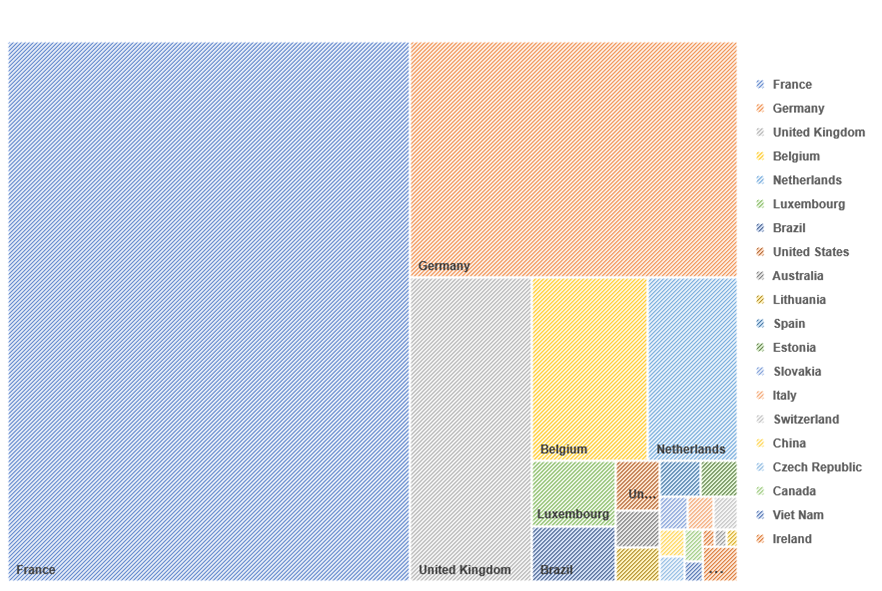
\includegraphics[width=10.3cm]{./pictures/monarc-countries-estimation.png}
      \end{figure}
\end{frame}


\section{Democratization of risk analysis}
\begin{frame}
    \frametitle{MONARC}
    \framesubtitle{Democratization of risk analysis}
    \begin{center}
        \begin{itemize}
            \item we are always open to comments for improvements;
            \item we are devoted to help and secure small businesses;
            \item we want uncompromising simple, fast and cost-effective risk analysis;
            \item \url{https://my.monarc.lu} is the free service based on MONARC (currently the host of approximately 260 independant instances).
        \end{itemize}
    \end{center}
\end{frame}



\section*{Conclusion}
\begin{frame}
    \frametitle{Interoperability by sharing knowledge}
    \begin{center}
        Interoperability can only be achieved by sharing information with open source
        software, interoperability of data and a common vocabulary.
    \end{center}
\end{frame}


%
% SECTION: End of the presentation
%
\section*{End of the presentation}
\begin{frame}
    \frametitle{End of the presentation}
    \framesubtitle{}
    \begin{center}
        \begin{itemize}
            \item Thank you for listening.
            \item Contact: info@cases.lu
            \item \url{https://github.com/CASES-LU}
            \item \url{https://github.com/monarc-project}
            \item \url{https://www.monarc.lu}
        \end{itemize}
    \end{center}
\end{frame}
\end{document}
